\documentclass[../dissertation.tex]{subfiles}

\begin{document}

For minimising a differentiable function $f:E \subset \mathbb{R}^n \rightarrow \mathbb{R}$, there is a well-known method known as \textbf{steepest descent method} (SDM)\cite{doi:10.1137/1.9781611974997.ch8}.
\begin{equation}
    \xbf^{k+1} = \xbf^{k} - \alpha_k \nabla f \left( \xbf^{k} \right)
    \label{equ: SDM}
\end{equation}
Starting from the initial input point $\xbf^{0}$, at each iteration, input points $\left\{ \xbf^{k} \right\}$ move in the direction of ``steepest'' decrease,
with specified step size $\alpha_k > 0$,
reducing the value at evaluation of $f$.
\begin{figure}[tbp]
    \centering
    \begin{subfigure}[b]{0.4\textwidth}
        \centering
        \includegraphics[width=\textwidth]{sections/gradientFlowImgs/sdm}
        \caption{SDM applied to $f(x,y) = -3 \cos x + \cos^2 y$ at different initial points.}
        \label{fig: SDM}
    \end{subfigure}
    \hspace{1cm}
    \begin{subfigure}[b]{0.4\textwidth}
        \centering
        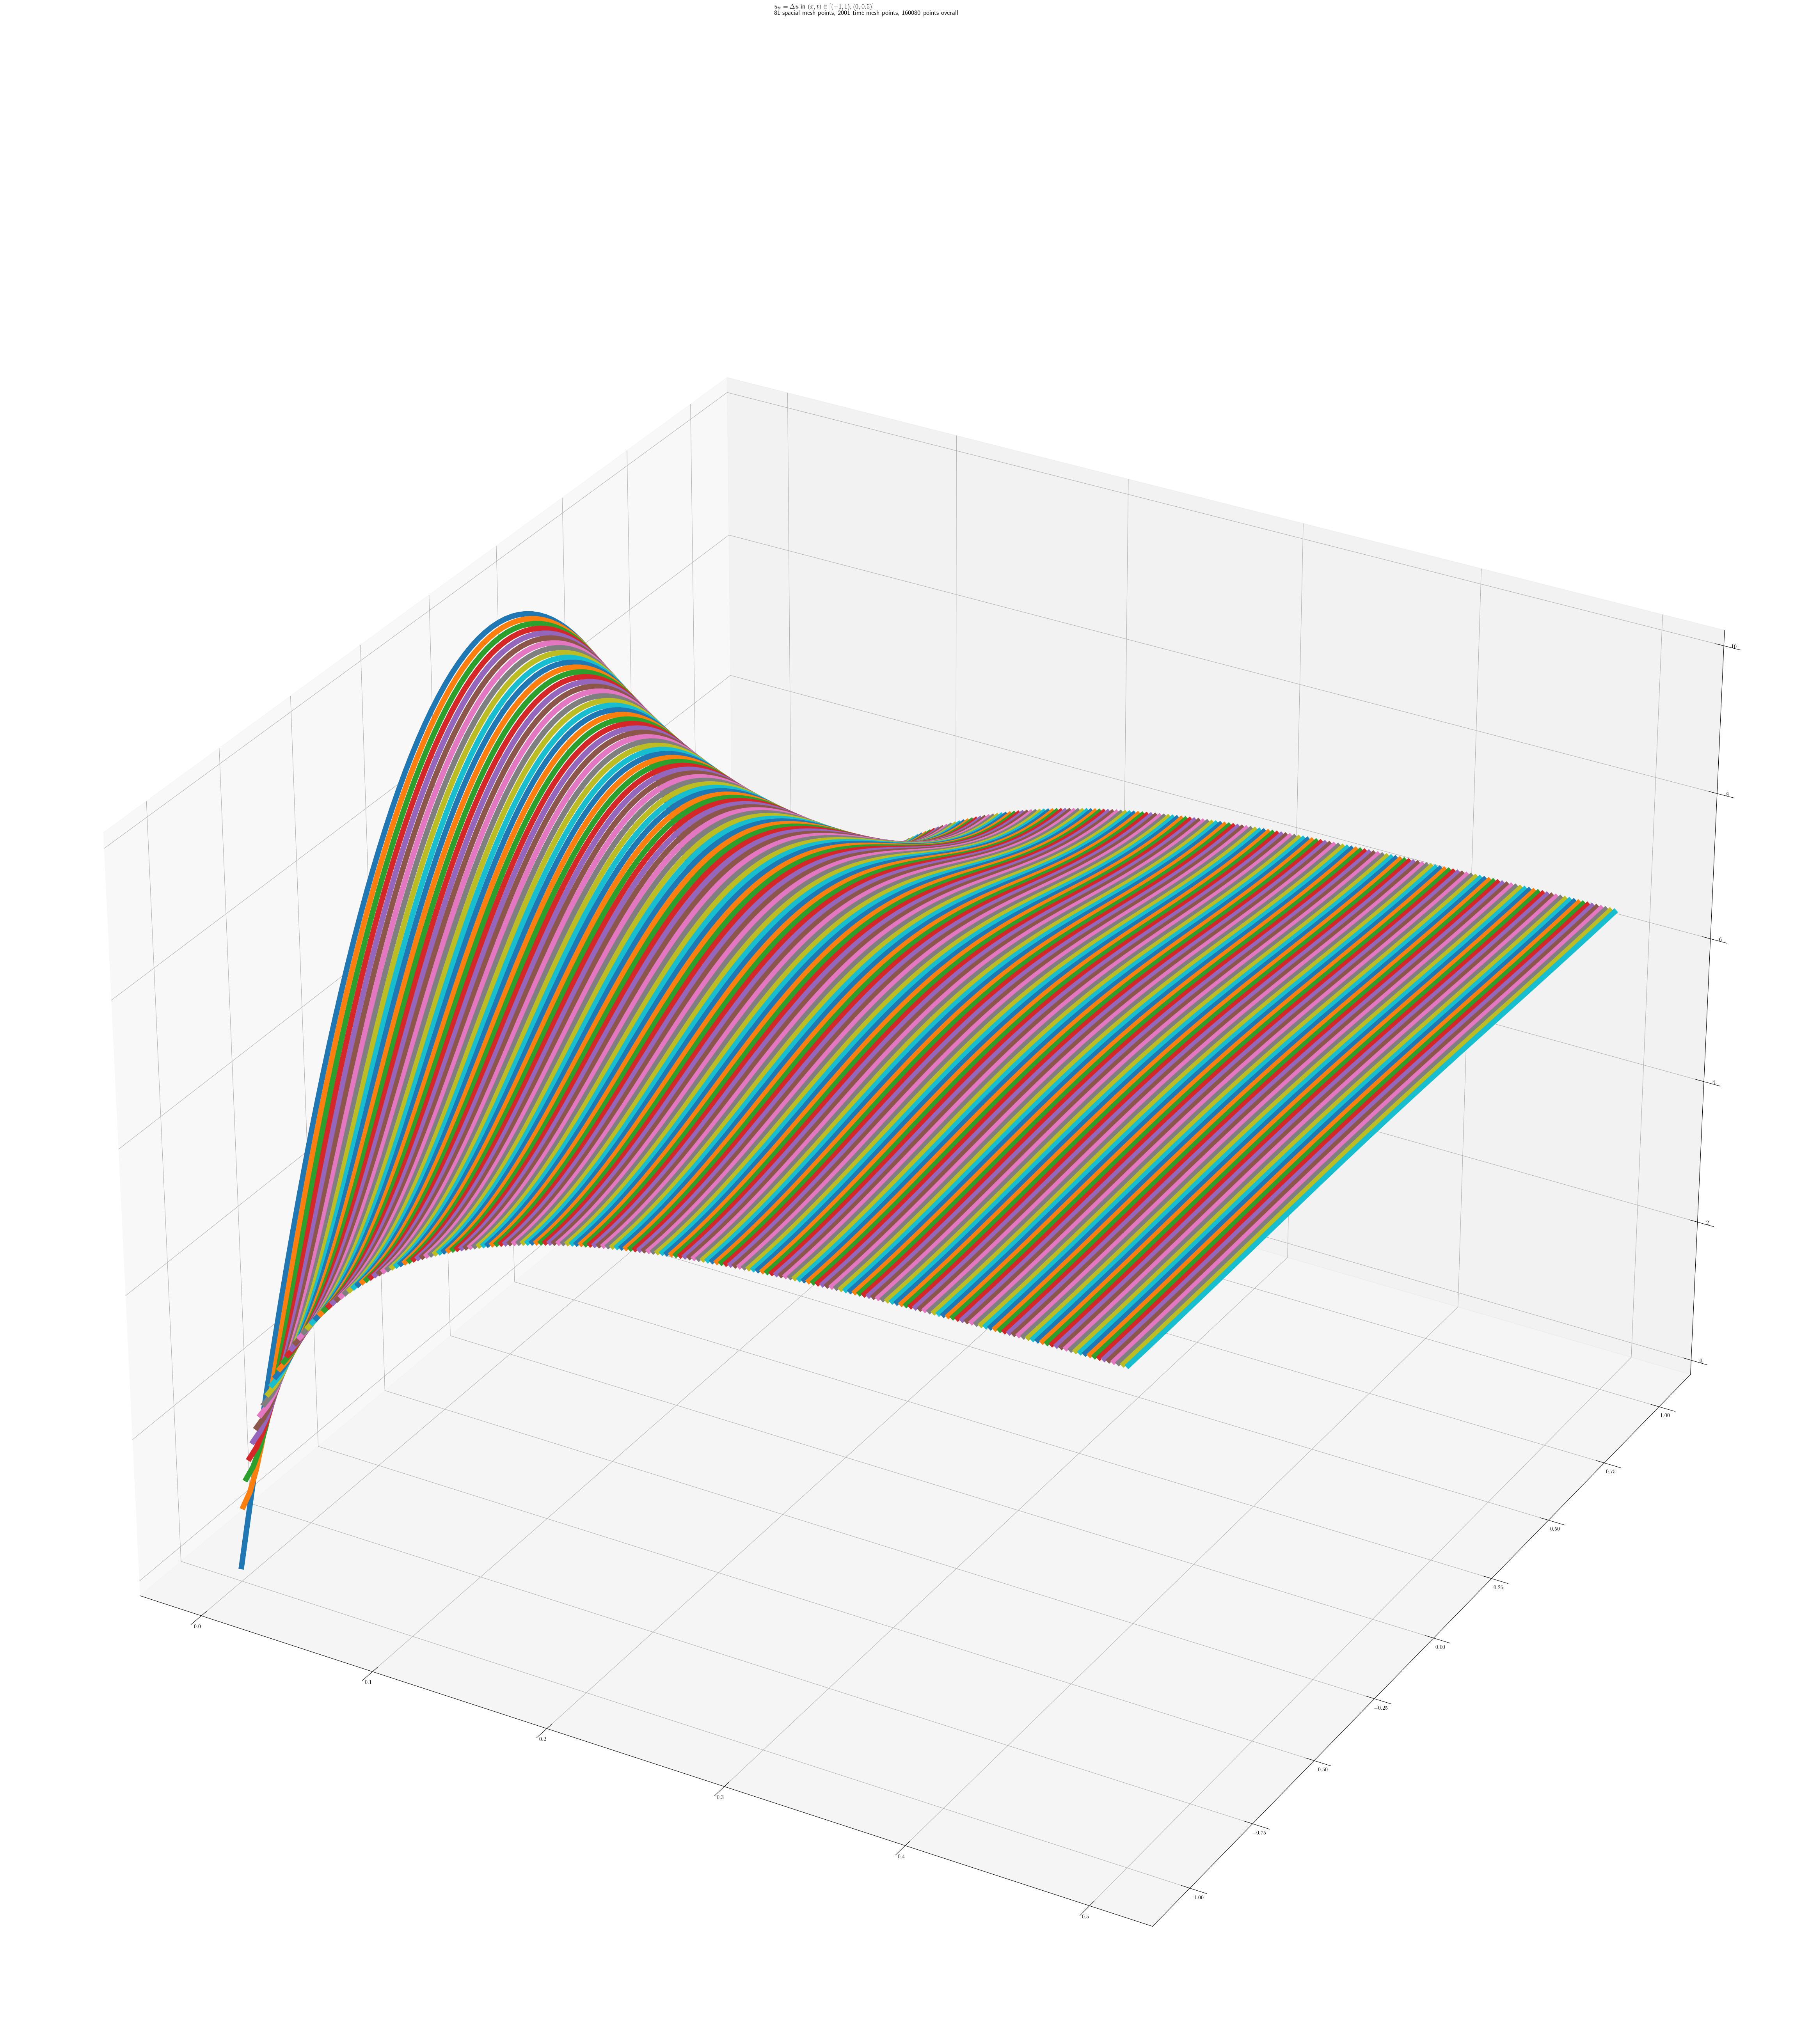
\includegraphics[width=\textwidth]{sections/gradientFlowImgs/gf}
        \caption{Solution to $L^2$ gradient flow equation with 1D energy functional $\mathcal{E} (f) \coloneqq \int_{-1}^1 \abs{\nabla f(x)}^2 \intd x$, which penealises variation in function. Note that the solution converges to a function with no variation.}
        \label{fig: GF}
    \end{subfigure}
    \caption{Gradient flow can be understood as a continuous analogue of steepest descent.}
\end{figure}
Note that in general, this method is not guaranteed to find the minimiser as shown in Figure (\ref{fig: SDM}).
On the other hand, convergence is guaranteed under certain assumptions, for example, convexity and $L$-smoothness\footnote{$\norm{\nabla f(\xbf) - \nabla f(\ybf)} \leq L \norm{\xbf-\ybf}$ for some constant $L > 0$}
with a certain choice of step size $\alpha_k$.

Analogously, differential equation known describing the reduction process of a functional $F:\mathcal{X} \rightarrow \mathbb{R}$ (where $\mathcal{X}$ is an inner product function space) can be motivated.
Starting from (\ref{equ: SDM}), replacing $\xbf^{k}$ by $f_k$ and $\nabla f\left( \xbf^k \right)$ by $\grad_{\mathcal{X}} F\left( f_k \right)$
\begin{equation}
    f_{k+1} = f_k - \alpha_k \grad_{\mathcal{X}} F \left( f_k \right)
    \label{equ: Gradient Flow Motivation}
\end{equation}
Now think of $f_k$ as ``snapshots'' at certain time $t = t_k$.
Without loss of generality, let $\alpha_k \equiv 1$.\footnote{
This is justified by taking a differrent time scale; essentially nondimensionalisation.
Also $\alpha_k \sim O (1)$ as $k \rightarrow \infty$ (eg. $\alpha = L^{-1}$ for $L$-smooth optimisation) is in fact a realistic choice.}
Dividing (\ref{equ: Gradient Flow Motivation}) by time step $\Delta t \coloneqq t_{k+1} - t_k$,
and taking the limit as $\Delta t \rightarrow 0$,
we acquire the \textbf{gradient flow equation}\cite{YSC2021}.
\begin{equation}
    \frac{\partial f}{\partial t} = - \grad_{\mathcal{X}} F (f)
    \label{equ: Gradient Flow Equation}
\end{equation}
where index $k$ transforms to ``time'' variable $t$.

Note that $\grad$ of a functional is not defined yet. This depends on the inner product function space $\mathcal{X}$ (eg. $L^2$, $H^1$, \ldots) of interest.

\end{document}
